\documentclass[preview]{standalone}

\usepackage{amsmath}
\usepackage{amssymb}
\usepackage{stellar}
\usepackage{bettelini}
\usepackage{makecell}
\usepackage{tikz}

\usetikzlibrary{decorations.pathreplacing}

\hypersetup{
    colorlinks=true,
    linkcolor=black,
    urlcolor=blue,
    pdftitle={Stellar},
    pdfpagemode=FullScreen,
}

\begin{document}

\title{Geografia economica}
\id{geoeconomica-globalizzazione}
\genpage

\section{Globalizzazione}

\begin{snippetdefinition}{globalizzazione-definition}{Globalizzazione}
    La \textit{globalizzazione} è un fenomeno che coinvolge l'interconnessione e l'interdipendenza crescente tra le nazioni e le persone in tutto il mondo.
\end{snippetdefinition}

\begin{snippet}{globalizzazione-expl}
    La globalizzazione porta su scala mondiale un incentramento di aspetti economici, sociali, culturali e politici.

    I terminini \textbf{multinazionale} e \textbf{transnazionale} hanno spesso
    un'accezione comune ma possono essere distinti nella seguente maniera
    \begin{itemize}
        \item \textbf{Multinazionale:} si riferisce a un'azienda o un'impresa che
            ha operazioni o filiali in più di un paese.
            Queste aziende hanno una presenza globale e conducono attività in diverse nazioni,
            ma il termine non necessariamente implica che l'azienda sia completamente interconnessa
            o integrata in tutte le operazioni.
            Le multinazionali possono avere sedi in diversi paesi,
            ma le decisioni strategiche e operative possono rimanere decentralizzate.
            \item \textbf{Transnazionale:} si riferisce a un'entità o un'organizzazione che opera
            al di là dei confini nazionali.
            Questo concetto si concentra sull'idea di superare le frontiere nazionali
            e lavorare in un contesto globale,
            con un'accentuata integrazione delle operazioni e delle decisioni su scala internazionale.
            Le aziende transnazionali tendono a essere più interconnesse e
            integrate rispetto alle multinazionali e spesso cercano di operare
            in un modo che superi le limitazioni geografiche e politiche.
    \end{itemize}
\end{snippet}

\begin{snippet}{polarismo-illustration}
    %=== GRAFICO POLARISMO ===
    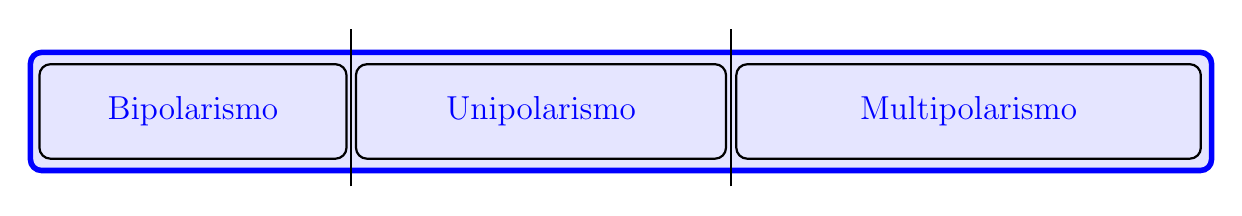
\begin{tikzpicture}
        \tikzset{box style/.style={draw, thick, rectangle, rounded corners, fill=blue!10, text=blue, font=\fontsize{12}{14}\selectfont}}
        \tikzset{line style/.style={line width=2pt, color=blue}}

        \draw[line style, fill=blue!10, rounded corners] (0,0) rectangle (15,1.5);
        \draw[thick] (4.075,-0.2) -- (4.075,1.8);
        \draw[thick] (8.9,-0.2) -- (8.9,1.8);

        \node[box style, anchor=west, minimum width=3.9cm, minimum height=1.2cm] at (0.1, 0.75) {Bipolarismo};
        \node[box style, anchor=west, minimum width=4.7cm, minimum height=1.2cm] at (4.12, 0.75) {Unipolarismo};
        \node[box style, anchor=west, minimum width=5.9cm, minimum height=1.2cm] at (8.95, 0.75) {Multipolarismo};
    \end{tikzpicture}

    %=== GRAFICO MULTILATERALISMO ===
    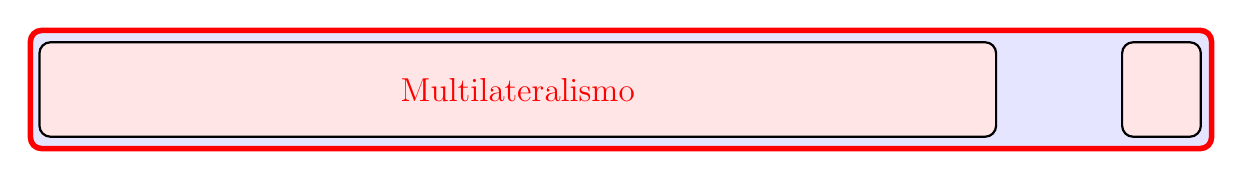
\begin{tikzpicture}
        \tikzset{box style/.style={draw, thick, rectangle, rounded corners, fill=red!10, text=red, font=\fontsize{12}{14}\selectfont}}
        \tikzset{line style/.style={line width=2pt, color=red}}

        \draw[line style, fill=blue!10, rounded corners] (0,0) rectangle (15,1.5);

        \node[box style, anchor=west, minimum width=12.15cm, minimum height=1.2cm] at (0.1, 0.75) {Multilateralismo};
        \node[box style, anchor=west, minimum width=1cm, minimum height=1.2cm] at (13.85, 0.75) {};
    \end{tikzpicture}
        %=== LINEA DEL TEMPO ===
    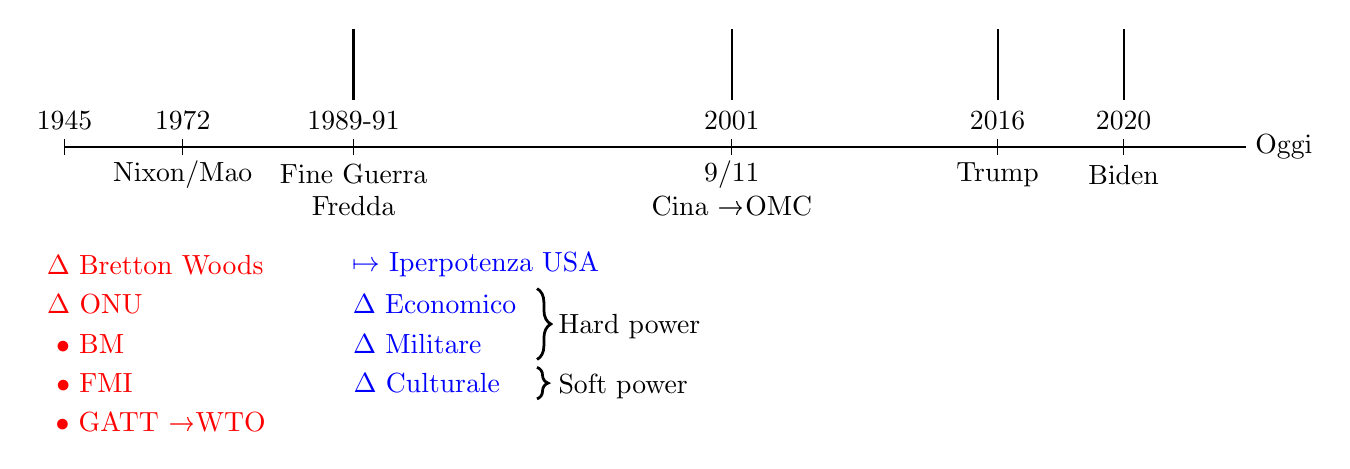
\begin{tikzpicture}
        \draw[thick] (0,0) -- (15,0);

        \foreach \x/\text in {0/1945, 1.5/1972, 3.67/1989-91, 8.475/2001, 11.85/2016, 13.45/2020}
            \draw (\x,-0.1) -- (\x,0.1) node[above] {\text};

        \node at (1.5,-0.35) {Nixon/Mao};
        \node at (3.67,-0.35) {Fine Guerra};
        \node at (3.67,-0.75) {Fredda};
        \draw[thick] (3.67,0.6) -- (3.67,1.5);
        \node at (8.475,-0.35) {9/11};
        \node at (8.475,-0.75) {Cina \textrightarrow OMC};
        \draw[thick] (8.475,0.6) -- (8.475,1.5);
        \node at (11.85,-0.35) {Trump};
        \draw[thick] (11.85,0.6) -- (11.85,1.5);
        \node at (13.45,-0.35) {Biden};
        \draw[thick] (13.45,0.6) -- (13.45,1.5);
        \node at (15,0) [right] {Oggi};

        %=== Legenda 1945 ===
        {\color{red}
        \node at (1.15,-1.5) {$\Delta$ Bretton Woods};
        \node at (0.385,-2) {$\Delta$ ONU};
        \node at (0.325,-2.5) {$\bullet$ BM};
        \node at (0.38,-3) {$\bullet$ FMI};
        \node at (1.22,-3.5) {$\bullet$ GATT \textrightarrow WTO};
        }

        %=== Legenda 1989 ===
        {\color{blue}
        \node at (5.22,-1.5) {$\mapsto$ Iperpotenza USA};
        \node at (4.7,-2) {$\Delta$ Economico};
        \node at (4.48,-2.5) {$\Delta$ Militare};
        \node at (4.6,-3) {$\Delta$ Culturale};
        }
        
        \draw[decorate, decoration={brace, amplitude=5pt, mirror}, line width=1pt] 
        (6,-2.7) -- (6,-1.8) node [black,midway,xshift=-0.6cm] {};
        \node[align=left, anchor=west] at (6.15, -2.28) {Hard power};

        \draw[decorate, decoration={brace, amplitude=4pt, mirror}, line width=1pt] 
        (6,-3.2) -- (6,-2.8) node [black,midway,xshift=-0.6cm] {};
        \node[align=left, anchor=west] at (6.15, -3.05) {Soft power};
    \end{tikzpicture}
\end{snippet}

\end{document}